\vspace{\baselineskip}
\begin{figure}[H]
    \centering
    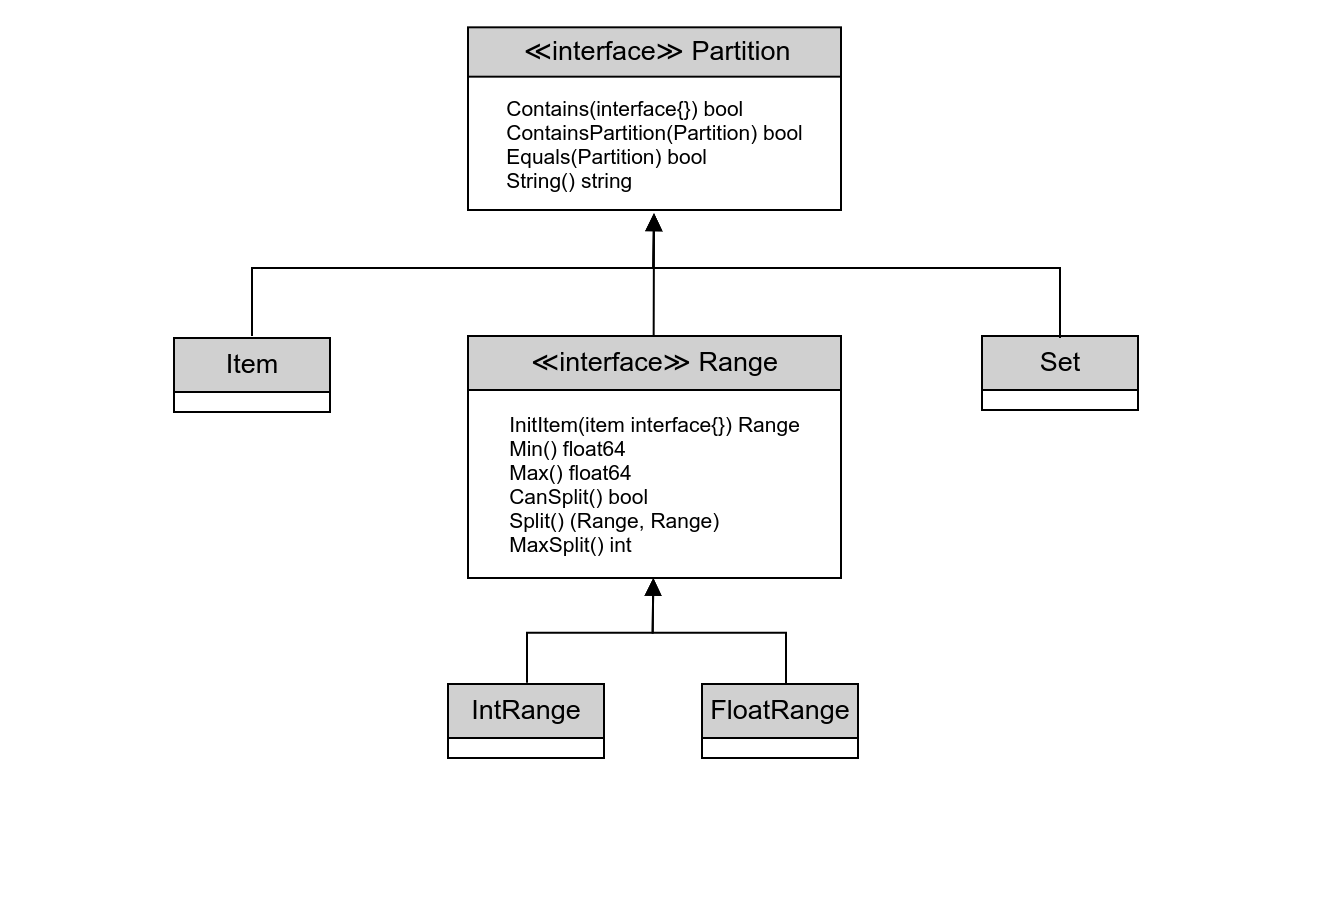
\includegraphics[width=\textwidth]{lib-partition.png}
    \caption{Partition hierarchy}\label{fig:partition_hierarchy}
\end{figure}


We have previously seen how partitions are the building blocks of generalization.
They are very similar to \textit{sets} in the mathematical sense.
In a standard generalization hierarchy we only needed to use \texttt{Partition}, \texttt{Item} and \texttt{Set}. (See Figure~\ref{fig:partition_hierarchy}.)

Representing larger ranges of numbers with the above strategy however would be very tedious.
We would not only have to write up each number on every level of the hierarchy, but also need to determine at what number the ranges are split up into partitions, and assign the proper parent-child relationships.
It is too much work, and in case of floating point numbers not even possible.
One option could be to generate a hierarchy with a \texttt{HierarchBuilder} as mentioned in~\ref{subsec:hierarchy_generalizer}. This removes the manual work of building up the partitions, but still has the need to store the whole hierarchy in the memory. For very large sets this could be inefficient.
We need a more feasible way of describing these types of dimensions.
This is why the \texttt{RangeGeneralizer} has been built into the library.

As it can be seen from Figure~\ref{fig:partition_hierarchy}, a \texttt{Range} interface can be derived from \texttt{Partition} which will deal with representing and splitting the ranges.
Its two implementations are \texttt{IntRange} and \texttt{FloatRange}.

The basic idea is, that after a number range is declared with its minimum and maximum boundaries, we can dynamically compute the partitions at the required level \emph{on the fly}.
Instead of keeping the full hierarchy in the memory, the \texttt{RangeGeneralizer} will \texttt{Split ()} the initial range the requested \texttt{n} number of times to arrive at the necessary generalization level.

\vspace{\baselineskip}
\vspace{\baselineskip}
\begin{figure}[H]
    \centering
    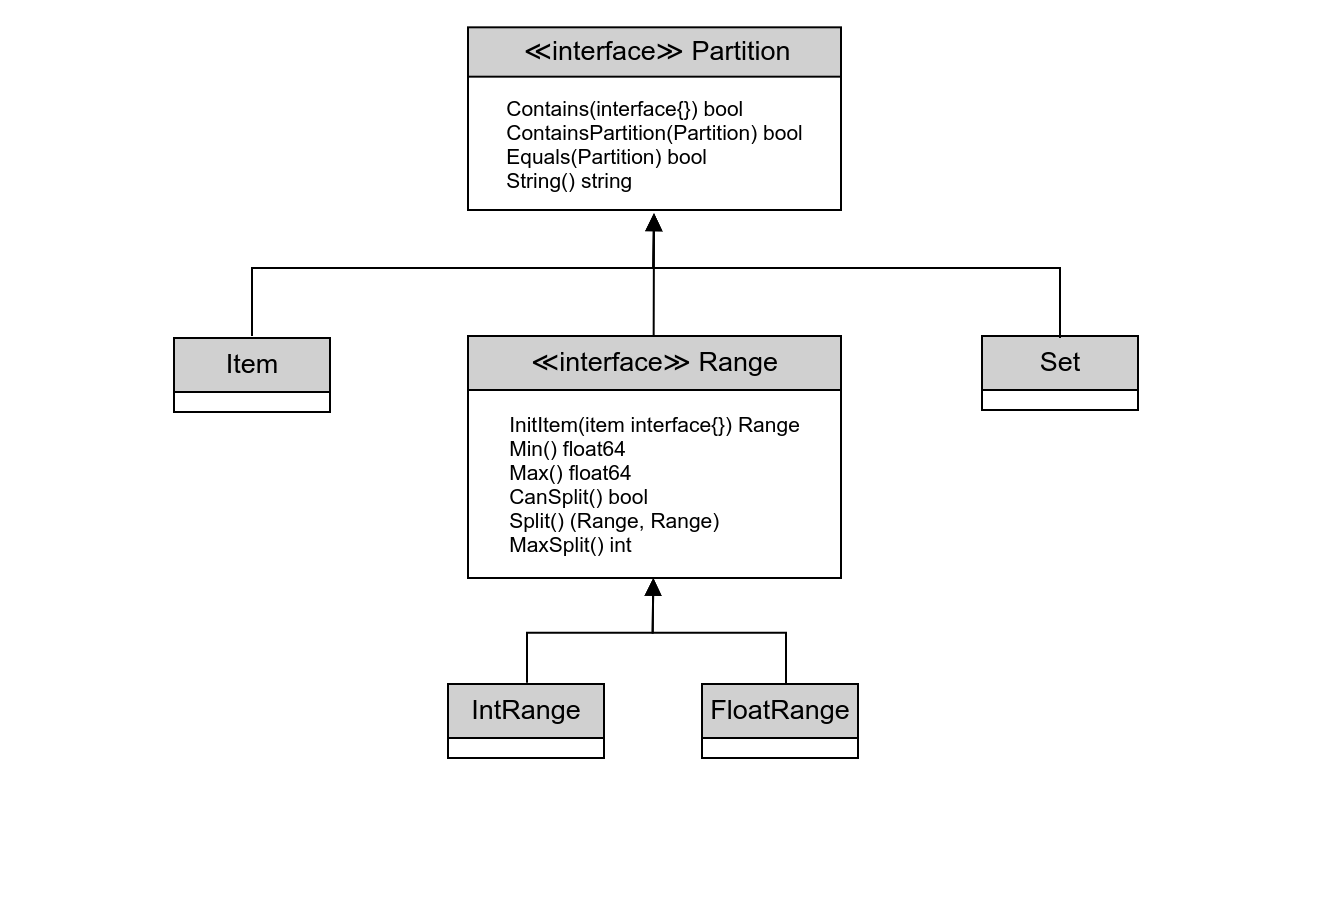
\includegraphics[width=\textwidth]{lib-partition.png}
    \caption{Partition hierarchy}\label{fig:partition_hierarchy}
\end{figure}


We have previously seen how partitions are the building blocks of generalization.
They are very similar to \textit{sets} in the mathematical sense.
In a standard generalization hierarchy we only needed to use \texttt{Partition}, \texttt{Item} and \texttt{Set}. (See Figure~\ref{fig:partition_hierarchy}.)

Representing larger ranges of numbers with the above strategy however would be very tedious.
We would not only have to write up each number on every level of the hierarchy, but also need to determine at what number the ranges are split up into partitions, and assign the proper parent-child relationships.
It is too much work, and in case of floating point numbers not even possible.
One option could be to generate a hierarchy with a \texttt{HierarchBuilder} as mentioned in~\ref{subsec:hierarchy_generalizer}. This removes the manual work of building up the partitions, but still has the need to store the whole hierarchy in the memory. For very large sets this could be inefficient.
We need a more feasible way of describing these types of dimensions.
This is why the \texttt{RangeGeneralizer} has been built into the library.

As it can be seen from Figure~\ref{fig:partition_hierarchy}, a \texttt{Range} interface can be derived from \texttt{Partition} which will deal with representing and splitting the ranges.
Its two implementations are \texttt{IntRange} and \texttt{FloatRange}.

The basic idea is, that after a number range is declared with its minimum and maximum boundaries, we can dynamically compute the partitions at the required level \emph{on the fly}.
Instead of keeping the full hierarchy in the memory, the \texttt{RangeGeneralizer} will \texttt{Split ()} the initial range the requested \texttt{n} number of times to arrive at the necessary generalization level.

\vspace{\baselineskip}
\vspace{\baselineskip}
\begin{figure}[H]
    \centering
    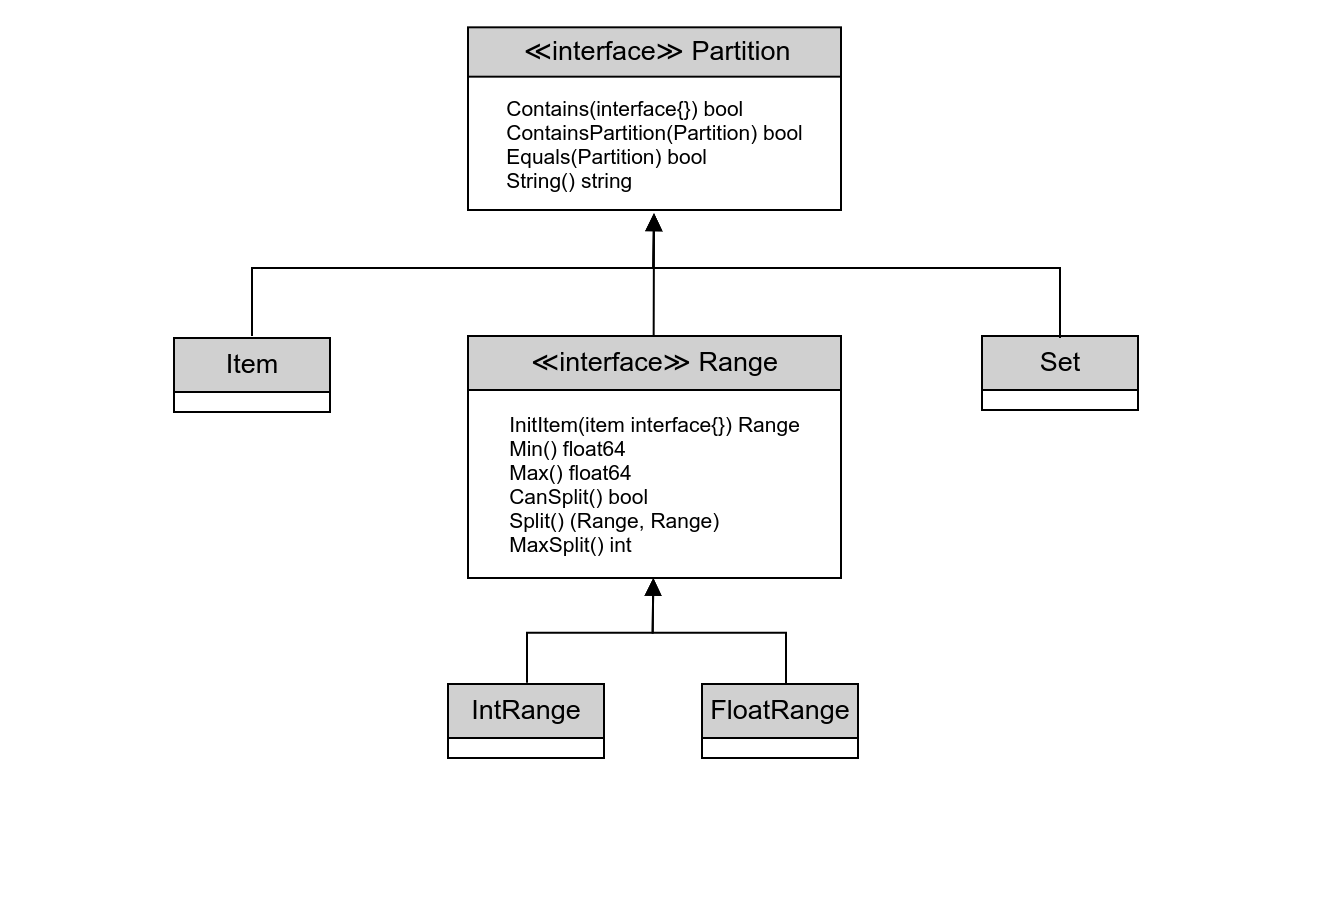
\includegraphics[width=\textwidth]{lib-partition.png}
    \caption{Partition hierarchy}\label{fig:partition_hierarchy}
\end{figure}


We have previously seen how partitions are the building blocks of generalization.
They are very similar to \textit{sets} in the mathematical sense.
In a standard generalization hierarchy we only needed to use \texttt{Partition}, \texttt{Item} and \texttt{Set}. (See Figure~\ref{fig:partition_hierarchy}.)

Representing larger ranges of numbers with the above strategy however would be very tedious.
We would not only have to write up each number on every level of the hierarchy, but also need to determine at what number the ranges are split up into partitions, and assign the proper parent-child relationships.
It is too much work, and in case of floating point numbers not even possible.
One option could be to generate a hierarchy with a \texttt{HierarchBuilder} as mentioned in~\ref{subsec:hierarchy_generalizer}. This removes the manual work of building up the partitions, but still has the need to store the whole hierarchy in the memory. For very large sets this could be inefficient.
We need a more feasible way of describing these types of dimensions.
This is why the \texttt{RangeGeneralizer} has been built into the library.

As it can be seen from Figure~\ref{fig:partition_hierarchy}, a \texttt{Range} interface can be derived from \texttt{Partition} which will deal with representing and splitting the ranges.
Its two implementations are \texttt{IntRange} and \texttt{FloatRange}.

The basic idea is, that after a number range is declared with its minimum and maximum boundaries, we can dynamically compute the partitions at the required level \emph{on the fly}.
Instead of keeping the full hierarchy in the memory, the \texttt{RangeGeneralizer} will \texttt{Split ()} the initial range the requested \texttt{n} number of times to arrive at the necessary generalization level.

\vspace{\baselineskip}
\vspace{\baselineskip}
\input{chapter03/figures/partition-hierarchy.tex}

We have previously seen how partitions are the building blocks of generalization.
They are very similar to \textit{sets} in the mathematical sense.
In a standard generalization hierarchy we only needed to use \texttt{Partition}, \texttt{Item} and \texttt{Set}. (See Figure~\ref{fig:partition_hierarchy}.)

Representing larger ranges of numbers with the above strategy however would be very tedious.
We would not only have to write up each number on every level of the hierarchy, but also need to determine at what number the ranges are split up into partitions, and assign the proper parent-child relationships.
It is too much work, and in case of floating point numbers not even possible.
One option could be to generate a hierarchy with a \texttt{HierarchBuilder} as mentioned in~\ref{subsec:hierarchy_generalizer}. This removes the manual work of building up the partitions, but still has the need to store the whole hierarchy in the memory. For very large sets this could be inefficient.
We need a more feasible way of describing these types of dimensions.
This is why the \texttt{RangeGeneralizer} has been built into the library.

As it can be seen from Figure~\ref{fig:partition_hierarchy}, a \texttt{Range} interface can be derived from \texttt{Partition} which will deal with representing and splitting the ranges.
Its two implementations are \texttt{IntRange} and \texttt{FloatRange}.

The basic idea is, that after a number range is declared with its minimum and maximum boundaries, we can dynamically compute the partitions at the required level \emph{on the fly}.
Instead of keeping the full hierarchy in the memory, the \texttt{RangeGeneralizer} will \texttt{Split ()} the initial range the requested \texttt{n} number of times to arrive at the necessary generalization level.

\vspace{\baselineskip}
\input{chapter03/figures/range-generalizer.tex}

Figure~\ref{fig:range_generalizer} shows an example of this in action. (Nodes with gray dotted border represent only a visual aid for the reader, the algorithm does not need to compute them.) Let's assume we are generalizing a range of integers \([0\dots10]\).
If we are interested in what partition the value \(n=4\) would be generalized into on level \(l=1\), we need to split the range \(s=l_{\max}-l-1=3\) times.
After each step we need to keep splitting the partition in which the requested element exists.
After the required number of splits we arrive at the result (partition \([3\dots4]\)) without having to worry about constructing the actual generalization hierarchy at any point.
Note, that the distribution of the items in the partitions is actually handled by how the \texttt{Split ()} function is implemented for the corresponding \texttt{Range}.
In this case (and in the library) we are using a uniform distribution by splitting each range at the median value.

With some modification this strategy can implemented for floating point ranges as well, but the code will need to take floating point precision into account, and compare with a delta.


Figure~\ref{fig:range_generalizer} shows an example of this in action. (Nodes with gray dotted border represent only a visual aid for the reader, the algorithm does not need to compute them.) Let's assume we are generalizing a range of integers \([0\dots10]\).
If we are interested in what partition the value \(n=4\) would be generalized into on level \(l=1\), we need to split the range \(s=l_{\max}-l-1=3\) times.
After each step we need to keep splitting the partition in which the requested element exists.
After the required number of splits we arrive at the result (partition \([3\dots4]\)) without having to worry about constructing the actual generalization hierarchy at any point.
Note, that the distribution of the items in the partitions is actually handled by how the \texttt{Split ()} function is implemented for the corresponding \texttt{Range}.
In this case (and in the library) we are using a uniform distribution by splitting each range at the median value.

With some modification this strategy can implemented for floating point ranges as well, but the code will need to take floating point precision into account, and compare with a delta.


Figure~\ref{fig:range_generalizer} shows an example of this in action. (Nodes with gray dotted border represent only a visual aid for the reader, the algorithm does not need to compute them.) Let's assume we are generalizing a range of integers \([0\dots10]\).
If we are interested in what partition the value \(n=4\) would be generalized into on level \(l=1\), we need to split the range \(s=l_{\max}-l-1=3\) times.
After each step we need to keep splitting the partition in which the requested element exists.
After the required number of splits we arrive at the result (partition \([3\dots4]\)) without having to worry about constructing the actual generalization hierarchy at any point.
Note, that the distribution of the items in the partitions is actually handled by how the \texttt{Split ()} function is implemented for the corresponding \texttt{Range}.
In this case (and in the library) we are using a uniform distribution by splitting each range at the median value.

With some modification this strategy can implemented for floating point ranges as well, but the code will need to take floating point precision into account, and compare with a delta.


Figure~\ref{fig:range_generalizer} shows an example of this in action. (Nodes with gray dotted border represent only a visual aid for the reader, the algorithm does not need to compute them.) Let's assume we are generalizing a range of integers \([0\dots10]\).
If we are interested in what partition the value \(n=4\) would be generalized into on level \(l=1\), we need to split the range \(s=l_{\max}-l-1=3\) times.
After each step we need to keep splitting the partition in which the requested element exists.
After the required number of splits we arrive at the result (partition \([3\dots4]\)) without having to worry about constructing the actual generalization hierarchy at any point.
Note, that the distribution of the items in the partitions is actually handled by how the \texttt{Split ()} function is implemented for the corresponding \texttt{Range}.
In this case (and in the library) we are using a uniform distribution by splitting each range at the median value.

With some modification this strategy can implemented for floating point ranges as well, but the code will need to take floating point precision into account, and compare with a delta.
